\documentclass[UTF8]{ctexart}
\CTEXsetup[format={\Large\bfseries}]{section}
\usepackage[a4paper,left=3cm,right=3cm,top=2cm]{geometry}
\usepackage{amsmath}
\usepackage{enumitem}
\usepackage{float}
\usepackage{threeparttable}
\usepackage{caption}
\usepackage{multirow}
\usepackage{graphicx}
\usepackage{listings}
\usepackage{color}
\definecolor{dkgreen}{rgb}{0,0.6,0}
\definecolor{gray}{rgb}{0.5,0.5,0.5}
\definecolor{mauve}{rgb}{0.58,0,0.82}
\lstset{frame=tb,
  language=html,
  aboveskip=3mm,
  belowskip=3mm,
  showstringspaces=false,
  columns=flexible,
  basicstyle={\small\ttfamily},
  numbers=left,%设置行号位置none不显示行号
  %numberstyle=\tiny\courier, %设置行号大小
  numberstyle=\tiny\color{gray},
  keywordstyle=\color{blue},
  commentstyle=\color{dkgreen},
  stringstyle=\color{mauve},
  breaklines=true,
  breakatwhitespace=true,
  escapeinside=`,%逃逸字符(1左面的键),用于显示中文例如在代码中`中文...`
  tabsize=4,
  extendedchars=false %解决代码跨页时,章节标题,页眉等汉字不显示的问题
}

\setlength\lineskiplimit{5.25bp}
\setlength\lineskip{5.25bp}

\title{数据分析及实践\ 实验二\ 实验报告}
\author{崔士强 PB22151743}
\date{\today}

\bibliographystyle{plain}

\begin{document}

\maketitle
\section*{任务1}
读取后得到的page.txt文件如图所示:
\begin{figure}[h]
  \centering
  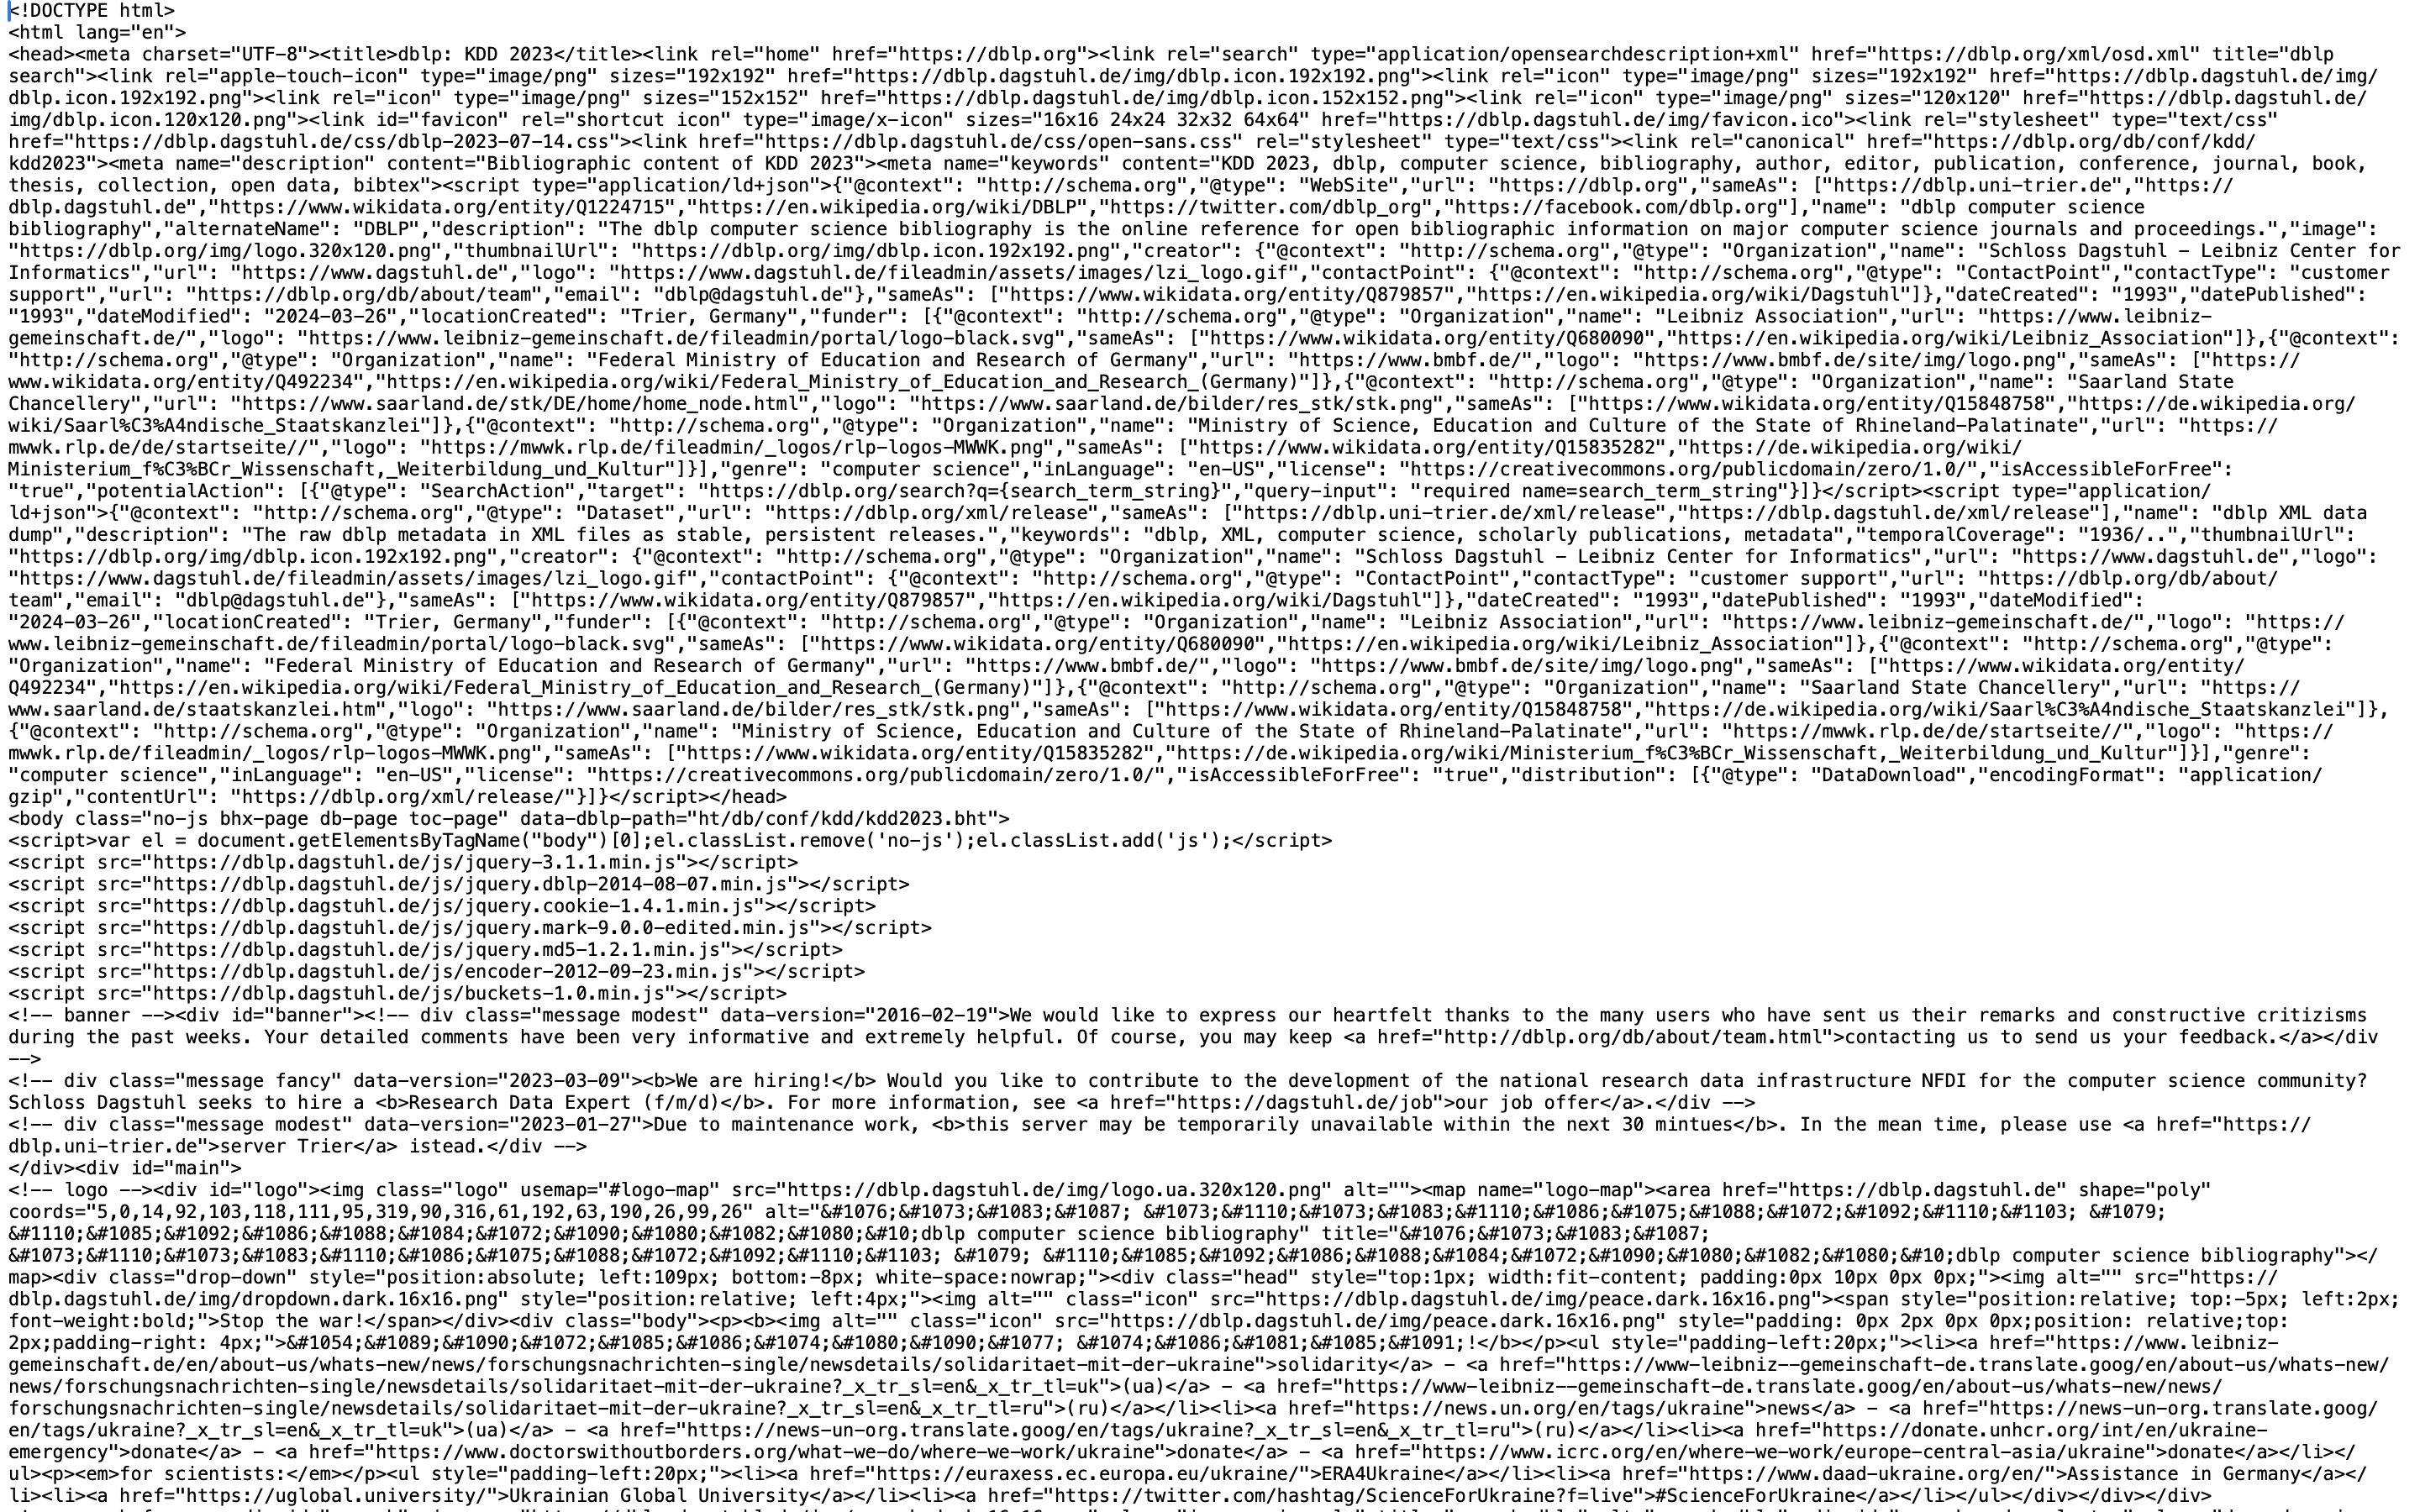
\includegraphics[scale=0.2]{page.png}
  \caption{page.txt文件内容}
\end{figure}

\section*{任务2}
通过观察可以发现,track名称跟在\lstinline|<h2 id=|后,对应设计正则表达式:
\begin{lstlisting}[language=python]
  title_pattern = '<h2 id=.{1,100}>.{1,100}</h2></header>'
\end{lstlisting}

输出5个track名称:
\begin{figure}[h]
  \centering
  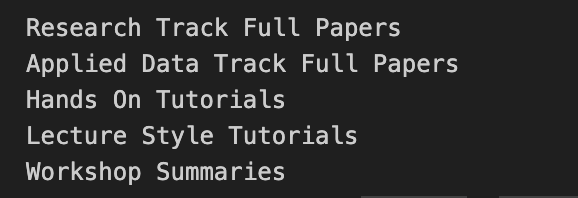
\includegraphics[scale=0.5]{tracks.png}
  \caption{各个track名称}
\end{figure}

\section*{任务3}
首先根据任务2中的规律,将字符串按track进行初步分割,再按照论文进一步分割. 对于目标元素,观察网页代码发现如下规律:
\begin{enumerate}
  \item 作者姓名在\lstinline|<span itemprop="name"|之后
  \item 论文标题在\lstinline|<span class="title" itemprop="name">|之后
  \item 收录起始页与终止页在\lstinline|<span itemprop="pagination">|之后
\end{enumerate}

对应设计正则表达式之后利用\lstinline{split()}方法取得目标字符串. 对论文进行
计数的结果如图所示
\begin{figure}[h]
  \centering
  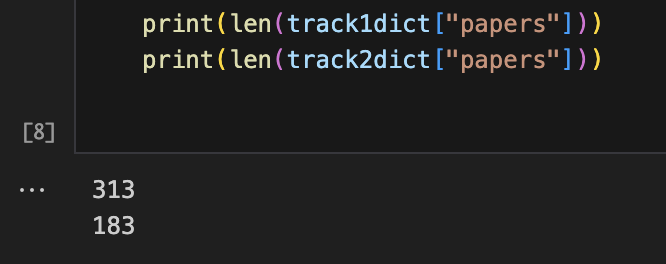
\includegraphics[scale=0.5]{count.png}
  \caption{两个track的论文计数}
\end{figure}

\section*{任务4}
存入\lstinline|kdd23.json|文件后如图所示
\begin{figure}[h]
  \centering
  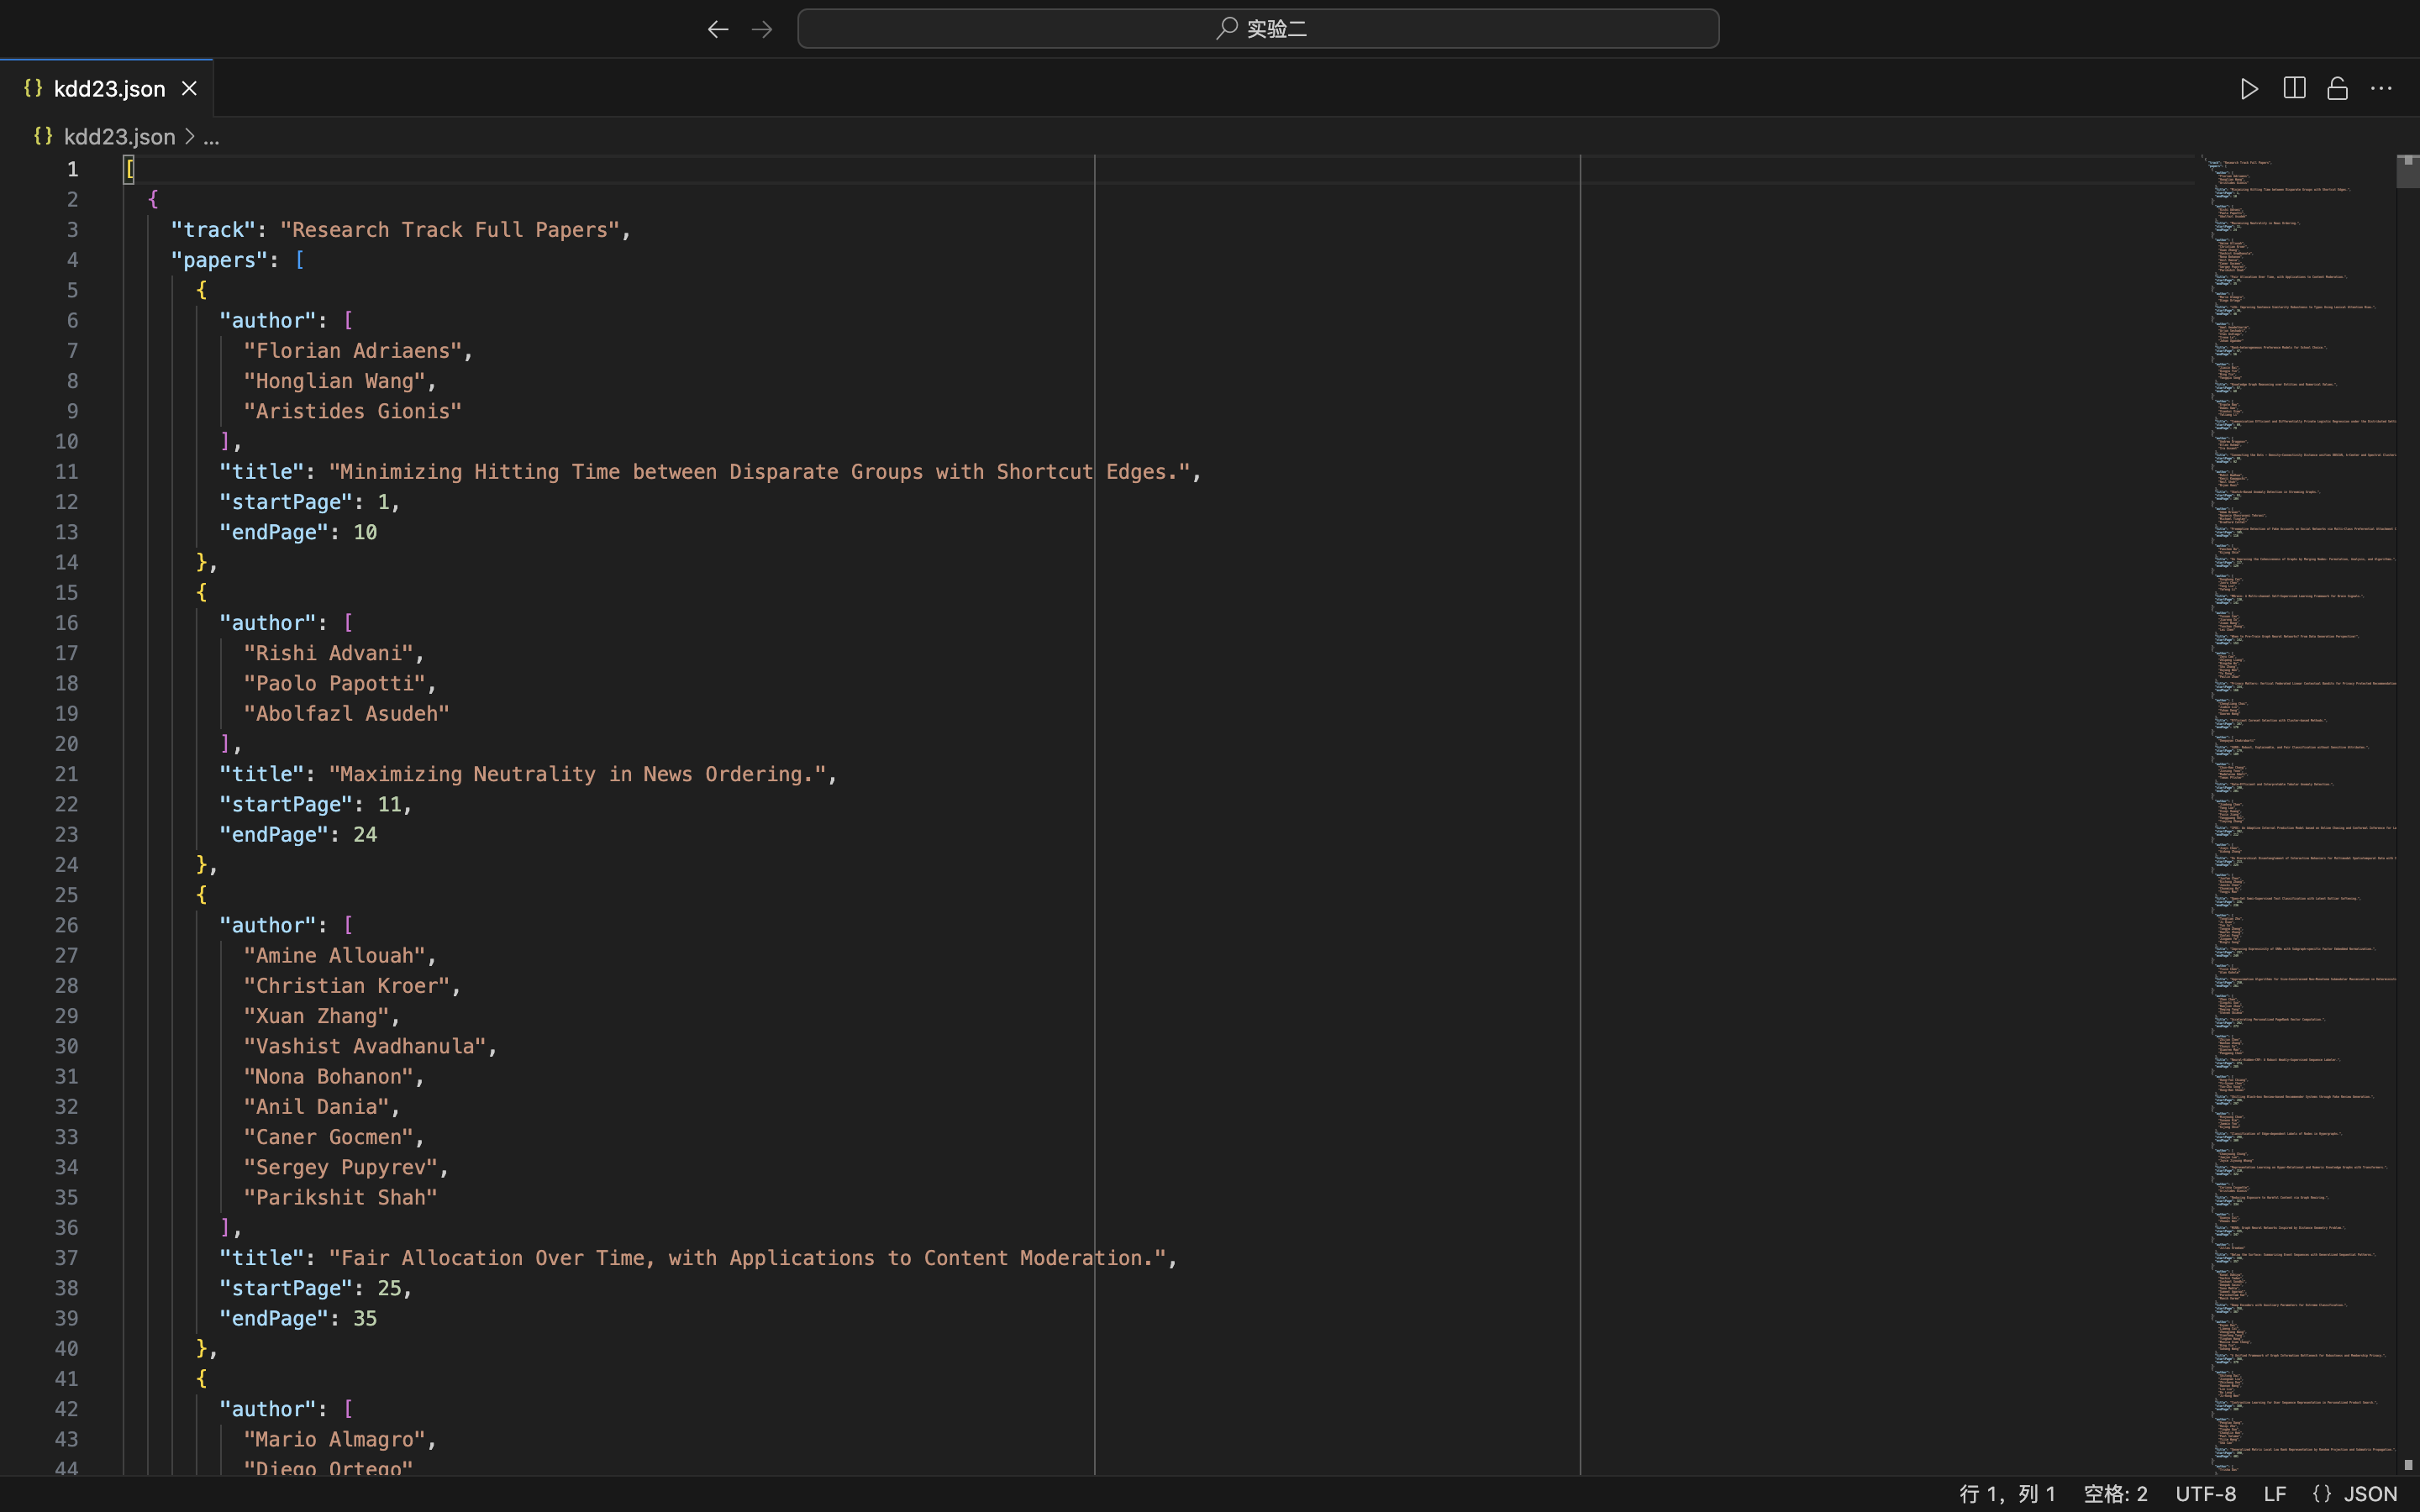
\includegraphics[scale=0.2]{kdd2023.png}
  \caption{kdd2023.json}
\end{figure}
\clearpage
\section*{任务5}
第一步是获取每个作者主页的链接,方法与任务3中大致相同. 之后利用\lstinline{request}库逐个
读取链接. 观察网页代码可以发现,\lstinline{publishInfo}可能包括: 1). \lstinline|volume|
2). \lstinline|issue| 3). \lstinline|pagination|. 因此逐个使用\lstinline|try...except|
语句查找,之后进行连接.

最后将信息写入\lstinline|researchers.json|文件,如图所示:
\begin{figure}[h]
  \centering
  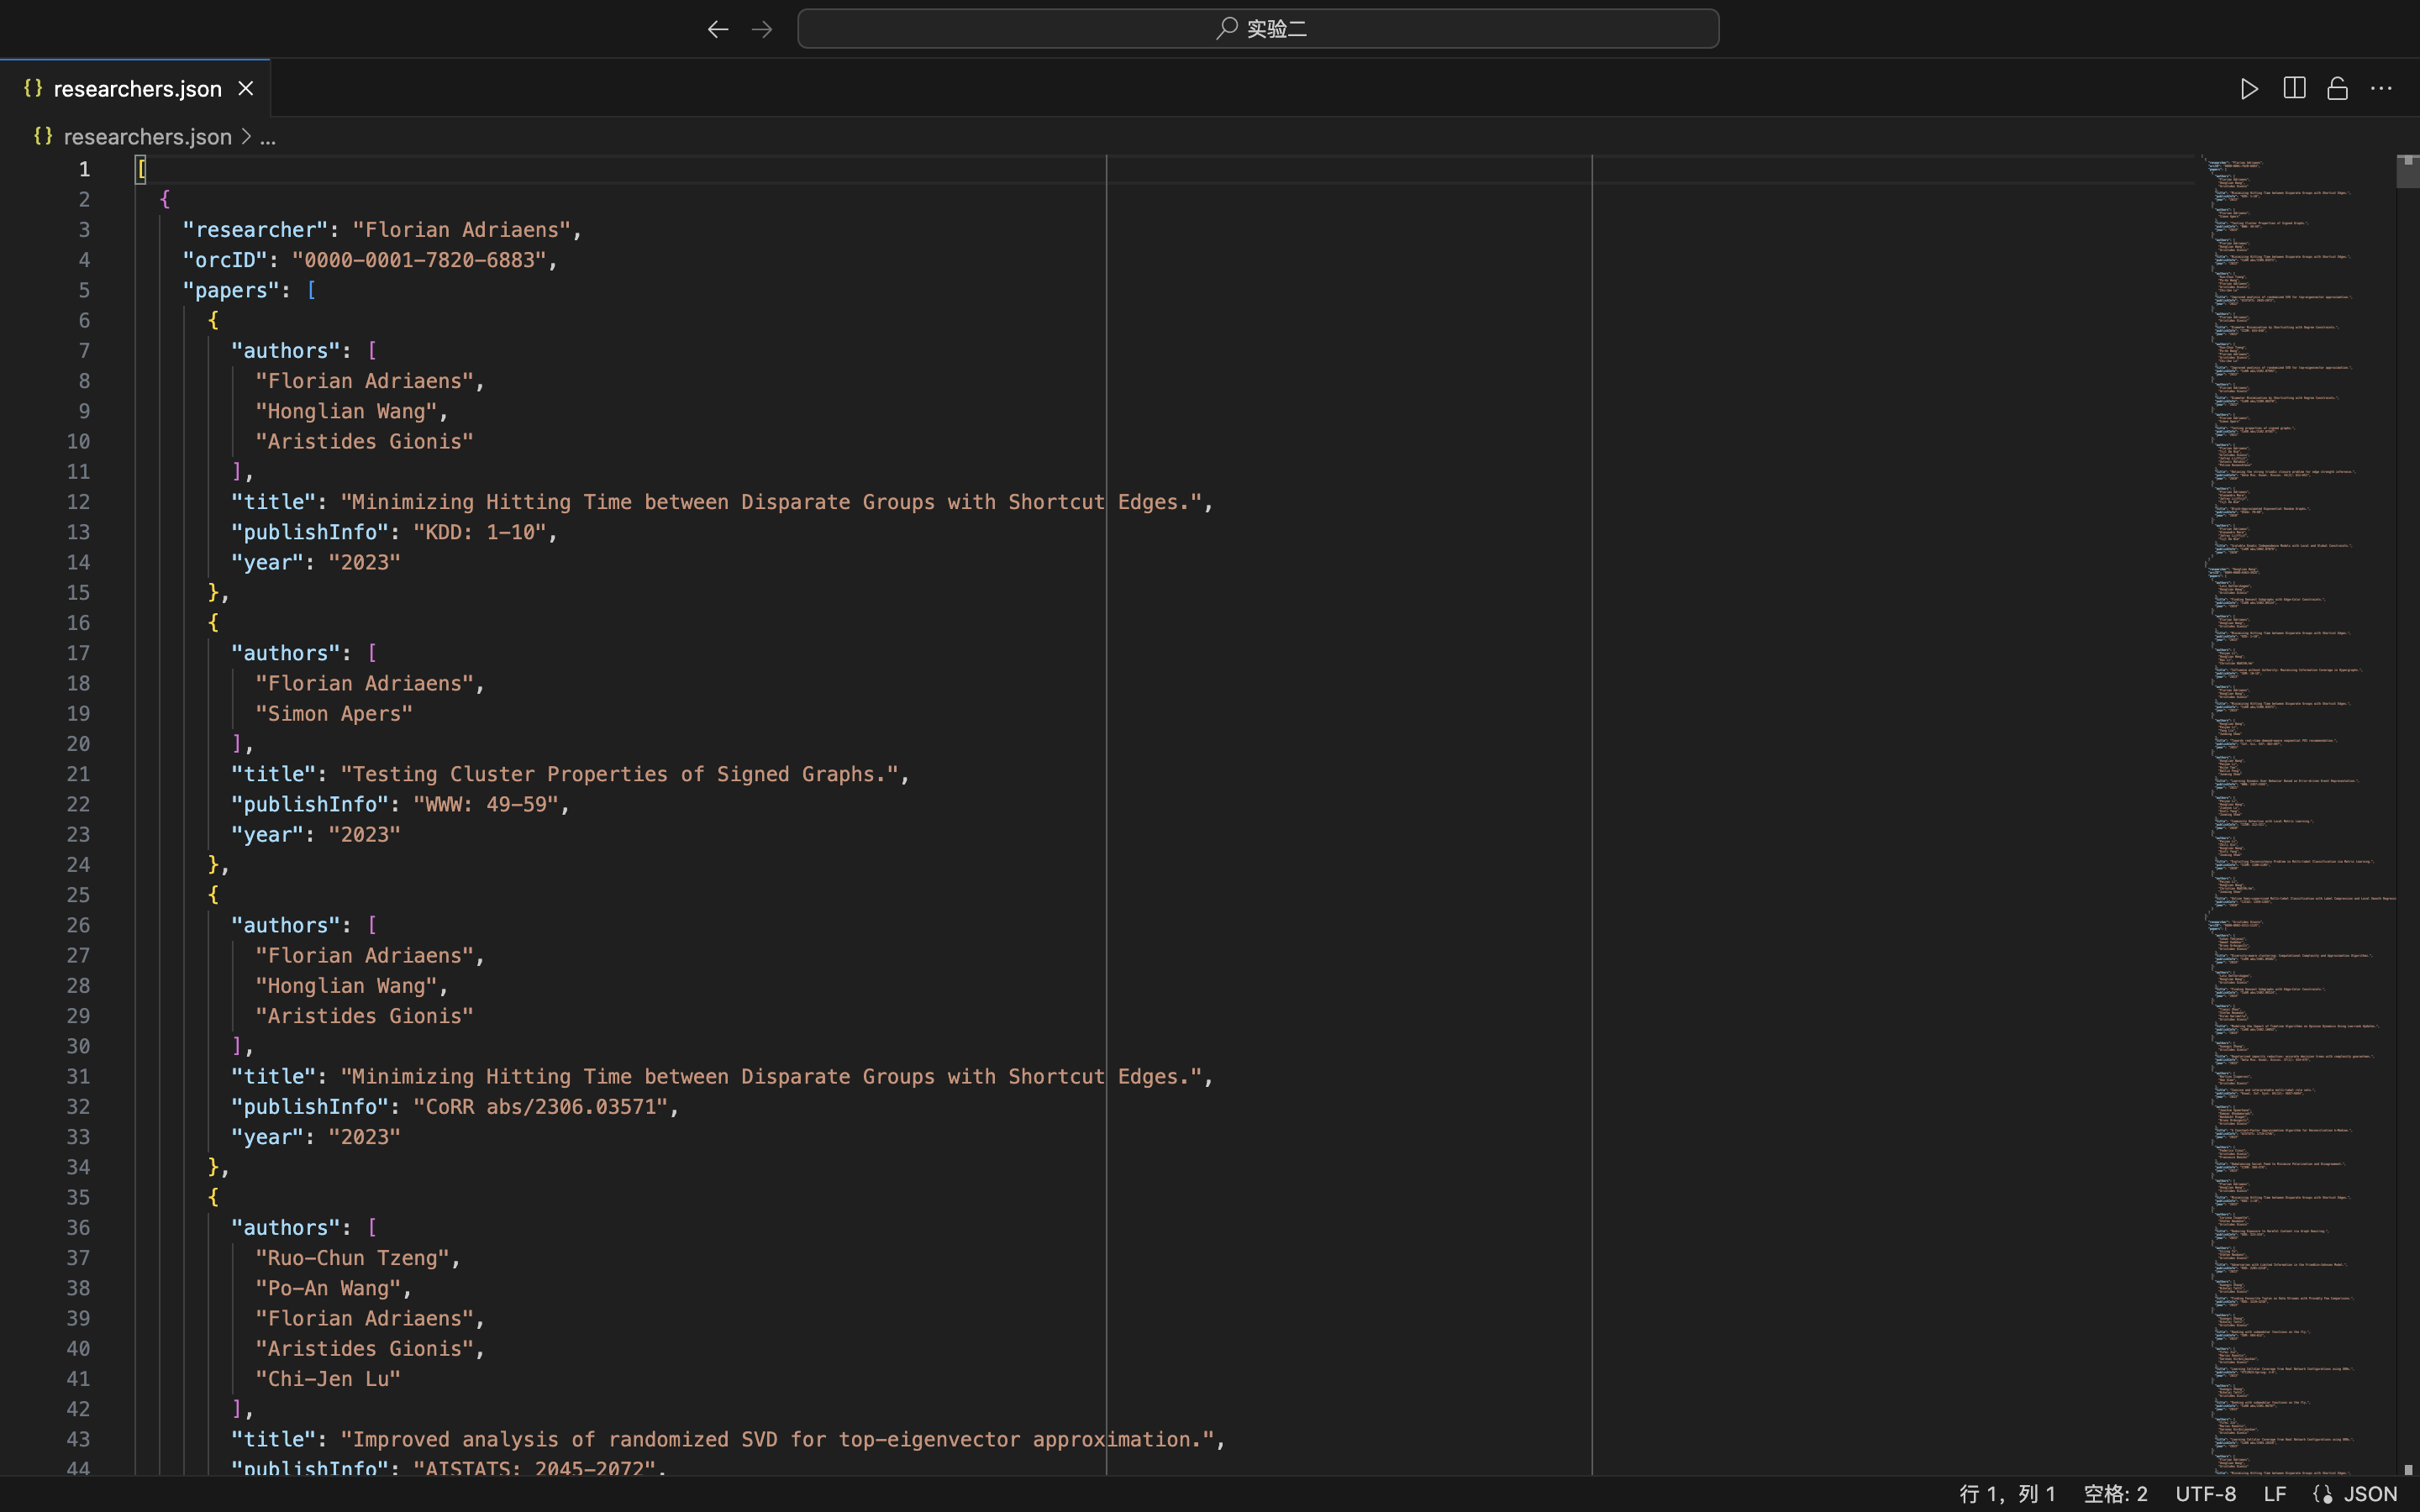
\includegraphics[scale=0.2]{researchers.png}
  \caption{name}
\end{figure}

\bibliography{math}

\end{document}
\iffalse
\begin{figure}[h]
    \centering
    \includegraphics[scale=0.5]{name.png}
    \caption{name}
\end{figure}
\fi
